\documentclass[tikz,border=4pt]{standalone}
\usepackage{tikz}
\usetikzlibrary{positioning, calc, arrows.meta, shapes.geometric}

\definecolor{mutblue}{RGB}{30,90,210}

\begin{document}
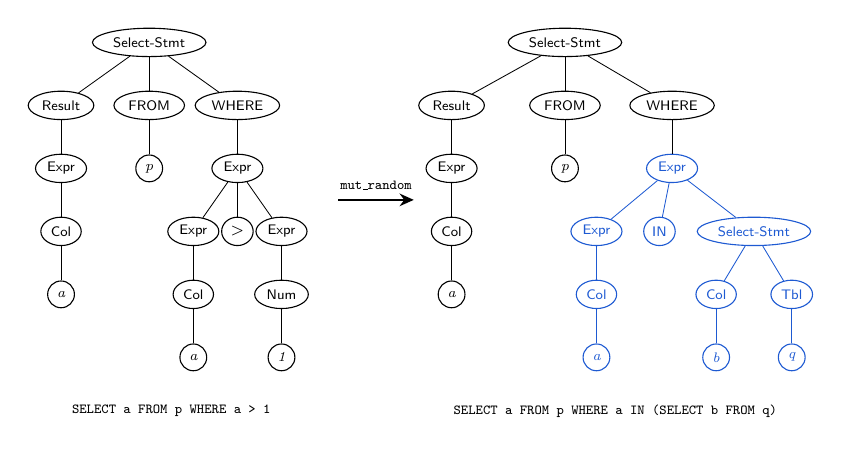
\begin{tikzpicture}[
    x=8mm, y=8mm,
    every node/.style={font=\tiny},
    % Non-terminal: small ellipse, snug fit
    nt/.style={ellipse, draw=black, line width=0.4pt,
        inner xsep=1.5pt, inner ysep=1pt, font=\tiny\sffamily,
        minimum height=3.6mm},
    % Operator: narrower ellipse
    op/.style={ellipse, draw=black, line width=0.4pt,
        inner xsep=0.5pt, inner ysep=1pt, font=\tiny\sffamily,
        minimum width=4mm, minimum height=3.6mm},
    % Leaf
    lf/.style={circle, draw=black, line width=0.4pt,
        inner sep=0pt, minimum size=3.4mm, font=\tiny\itshape},
    nth/.style={ellipse, draw=mutblue, line width=0.4pt,
        inner xsep=1.5pt, inner ysep=1pt, font=\tiny\sffamily,
        minimum height=3.6mm, text=mutblue},
    oph/.style={ellipse, draw=mutblue, line width=0.4pt,
        inner xsep=0.5pt, inner ysep=1pt, font=\tiny\sffamily,
        minimum width=4mm, minimum height=3.6mm, text=mutblue},
    lfh/.style={circle, draw=mutblue, line width=0.4pt,
        inner sep=0pt, minimum size=3.4mm, font=\tiny\itshape, text=mutblue},
    te/.style={draw=black, line width=0.3pt},
    teh/.style={draw=mutblue, line width=0.3pt},
    mutarrow/.style={-{Stealth[length=1.8mm,width=1.6mm]}, line width=0.6pt},
]

% ====== LEFT TREE: SELECT a FROM p WHERE a > 1 ======
\begin{scope}
    \node[nt] (L-root)   at (0, 0)     {Select-Stmt};

    \node[nt] (L-result) at (-1.4,-1)  {Result};
    \node[nt] (L-from)   at (0,-1)     {FROM};
    \node[nt] (L-where)  at (1.4,-1)   {WHERE};

    \node[nt] (L-expr1)  at (-1.4,-2)  {Expr};
    \node[lf] (L-p)      at (0,-2)     {p};
    \node[nt] (L-expr2)  at (1.4,-2)   {Expr};

    \node[nt] (L-col1)   at (-1.4,-3)  {Col};

    \node[nt] (L-expr3)  at (0.7,-3)   {Expr};
    \node[op] (L-gt)     at (1.4,-3)   {$>$};
    \node[nt] (L-expr4)  at (2.1,-3)   {Expr};

    \node[lf] (L-a1)     at (-1.4,-4)  {a};
    \node[nt] (L-col2)   at (0.7,-4)   {Col};
    \node[nt] (L-num)    at (2.1,-4)   {Num};

    \node[lf] (L-a2)     at (0.7,-5)   {a};
    \node[lf] (L-1)      at (2.1,-5)   {1};

    \foreach \a/\b in {L-root/L-result, L-root/L-from, L-root/L-where,
        L-result/L-expr1, L-from/L-p, L-where/L-expr2,
        L-expr1/L-col1,
        L-expr2/L-expr3, L-expr2/L-gt, L-expr2/L-expr4,
        L-col1/L-a1, L-expr3/L-col2, L-expr4/L-num,
        L-col2/L-a2, L-num/L-1}
        \draw[te] (\a) -- (\b);

    \node[font=\tiny\ttfamily, anchor=north] at (0.35,-5.6)
        {SELECT a FROM p WHERE a > 1};
\end{scope}

% ====== ARROW ======
\draw[mutarrow] (3.0,-2.5) -- node[above, font=\tiny\ttfamily] {mut\_random}
                              (4.2,-2.5);

% ====== RIGHT TREE: SELECT a FROM p WHERE a IN (SELECT b FROM q) ======
\begin{scope}[shift={(6.6,0)}]
    \node[nt] (R-root)   at (0,0)     {Select-Stmt};

    \node[nt] (R-result) at (-1.8,-1) {Result};
    \node[nt] (R-from)   at (0,-1)    {FROM};
    \node[nt] (R-where)  at (1.7,-1)  {WHERE};

    \node[nt]  (R-expr1) at (-1.8,-2) {Expr};
    \node[lf]  (R-p)     at (0,-2)    {p};
    \node[nth] (R-expr2) at (1.7,-2)  {Expr};

    \node[nt]  (R-col1)  at (-1.8,-3) {Col};

    \node[nth] (R-expr3) at (0.5,-3)  {Expr};
    \node[oph] (R-in)    at (1.5,-3)  {IN};
    \node[nth] (R-sel)   at (3.0,-3)  {Select-Stmt};

    \node[lf]  (R-a1)    at (-1.8,-4) {a};
    \node[nth] (R-col2)  at (0.5,-4)  {Col};
    \node[nth] (R-col3)  at (2.4,-4)  {Col};
    \node[nth] (R-tbl)   at (3.6,-4)  {Tbl};

    \node[lfh] (R-a2)    at (0.5,-5)  {a};
    \node[lfh] (R-b)     at (2.4,-5)  {b};
    \node[lfh] (R-q)     at (3.6,-5)  {q};

    \foreach \a/\b in {R-root/R-result, R-root/R-from, R-root/R-where,
        R-result/R-expr1, R-from/R-p, R-where/R-expr2,
        R-expr1/R-col1, R-col1/R-a1}
        \draw[te] (\a) -- (\b);
    \foreach \a/\b in {R-expr2/R-expr3, R-expr2/R-in, R-expr2/R-sel,
        R-expr3/R-col2, R-sel/R-col3, R-sel/R-tbl,
        R-col2/R-a2, R-col3/R-b, R-tbl/R-q}
        \draw[teh] (\a) -- (\b);

    \node[font=\tiny\ttfamily, anchor=north] at (0.8,-5.6)
        {SELECT a FROM p WHERE a IN (SELECT b FROM q)};
\end{scope}

\end{tikzpicture}
\end{document}